% =============================================================================
% supplement.tex -- Online Resource 1
% Compile: latexmk -pdf supplement.tex
% =============================================================================
\documentclass[11pt,a4paper]{article}
\usepackage[margin=22mm]{geometry}
\usepackage[utf8]{inputenc}
\usepackage[T1]{fontenc}
% \usepackage{lmodern}  % uncomment if the lmodern package is installed
\usepackage{amsmath}
\usepackage{graphicx}
\usepackage{booktabs}
\usepackage{longtable}
\usepackage{array}
\usepackage{float}
\usepackage{caption}
\usepackage[authoryear,round]{natbib}
\usepackage[hidelinks]{hyperref}
\usepackage{listings}
\usepackage{xcolor}
\graphicspath{{figures/}}
% panel helper: letter set in the document, not inside the image
\newcommand{\panel}[3]{\begin{minipage}[t]{#2}\raggedright\textbf{(#1)}\\[2pt]\includegraphics[width=\linewidth]{#3}\end{minipage}}

\captionsetup{labelfont=bf,labelsep=space,font=small}
\renewcommand{\figurename}{Fig.}
\renewcommand{\thetable}{S\arabic{table}}
\renewcommand{\thefigure}{S\arabic{figure}}
\bibliographystyle{plainnat}  % submit with spbasic (Springer); plainnat used for local build
\setcitestyle{aysep={}}
\lstset{basicstyle=\ttfamily\footnotesize,breaklines=true,frame=single,columns=fullflexible,
        backgroundcolor=\color{gray!8},language=R,keywordstyle=\color{blue!60!black},commentstyle=\color{gray!60!black}}
% results.tex -- GENERATED by scripts/make_results_macros.R. Do not edit.
% generated 2026-10-23 12:05:35.890232
\newcommand{\nScenarios}{108}
\newcommand{\nPanels}{120}
\newcommand{\nReplicates}{10}
\newcommand{\nDatasets}{1080}
\newcommand{\nFits}{5526}
\newcommand{\nFitsMain}{5400}
\newcommand{\waMax}{6.51}
\newcommand{\waCum}{192.7}
\newcommand{\waDur}{60}
\newcommand{\naiveBiasLagZero}{-0.016}
\newcommand{\naiveBiasLagOne}{0.065}
\newcommand{\naiveBiasLagTwo}{0.069}
\newcommand{\lagoneBiasLagZero}{0.058}
\newcommand{\lagoneBiasLagOne}{-0.016}
\newcommand{\lagoneBiasLagTwo}{0.065}
\newcommand{\dlnmBiasLagZero}{0.021}
\newcommand{\dlnmBiasLagOne}{-0.031}
\newcommand{\dlnmBiasLagTwo}{-0.004}
\newcommand{\gamBiasLagOne}{-0.039}
\newcommand{\naiveRelBiasLagOne}{79}
\newcommand{\naiveRelBiasLagTwo}{84}
\newcommand{\naiveRelBiasLagZero}{28}
\newcommand{\lagoneRelBiasLagOne}{27}
\newcommand{\lagoneRelBiasLagTwo}{79}
\newcommand{\dlnmRelBiasRange}{-45\% to 69\%}
\newcommand{\linearCoverageRange}{5\% to 7\%}
\newcommand{\naiveCoverage}{5\%}
\newcommand{\lagoneCoverage}{7\%}
\newcommand{\gamCoverage}{69\%}
\newcommand{\dlnmCoverage}{73\%}
\newcommand{\lagoneCoverageCorrectLag}{21\%}
\newcommand{\lagoneCoverageWrongLag}{0\%}
\newcommand{\dlnmCoverageMin}{54\%}
\newcommand{\dlnmCoverageMax}{92\%}
\newcommand{\dlnmCoverageLagOne}{54\%}
\newcommand{\gamCoverageLagOne}{100\%}
\newcommand{\gamCoverageMin}{42\%}
\newcommand{\naiveCoverageLagZero}{16\%}
\newcommand{\naiveCoverageLagOne}{0\%}
\newcommand{\dlnmSdLagOne}{0.025}
\newcommand{\lagoneSdLagOne}{0.004}
\newcommand{\naiveSdLagOne}{0.002}
\newcommand{\rfSdLagOne}{0.028}
\newcommand{\dlnmRmseLagOne}{0.051}
\newcommand{\dlnmRmseLagTwo}{0.027}
\newcommand{\lagoneRmseLagOne}{0.016}
\newcommand{\lagoneRmseLagTwo}{0.066}
\newcommand{\naiveRmseLagOne}{0.065}
\newcommand{\naiveLsLagZero}{-0.56}
\newcommand{\naiveLsLagOne}{-1.42}
\newcommand{\naiveLsLagTwo}{-1.87}
\newcommand{\lagoneLsLagZero}{-1.29}
\newcommand{\lagoneLsLagOne}{-1.03}
\newcommand{\lagoneLsLagTwo}{-1.83}
\newcommand{\gamLsLagOne}{-1.02}
\newcommand{\gamLsLagTwo}{-2.67}
\newcommand{\rfLsLagZero}{-0.61}
\newcommand{\rfLsLagOne}{-1.16}
\newcommand{\rfLsLagTwo}{-2.24}
\newcommand{\rfBiasLagOne}{0.007}
\newcommand{\rfBiasLagZero}{0.080}
\newcommand{\rfRelBiasLagOne}{-5}
\newcommand{\lagoneRelBiasWrongLag}{70\% and 79\%}
\newcommand{\dlnmRelBiasLagOne}{46}
\newcommand{\dlnmRelBiasLagZero}{-30}
\newcommand{\dlnmRelBiasLagTwo}{10}
\newcommand{\glmPctEstimate}{99.9}
\newcommand{\dlnmRmse}{0.036}
\newcommand{\naiveRmse}{0.030}
\newcommand{\lagoneRmse}{0.029}
\newcommand{\gamRmse}{0.053}
\newcommand{\rfRmse}{0.048}
\newcommand{\bestPredModel}{naive_glm}
\newcommand{\bestPredScore}{-1.28}
\newcommand{\naiveLogScore}{-1.28}
\newcommand{\lagoneLogScore}{-1.38}
\newcommand{\gamLogScore}{-1.60}
\newcommand{\rfLogScore}{-1.34}
\newcommand{\mainConvergedMin}{96.5}
\newcommand{\regionRankInvariant}{nearly identical}
\newcommand{\naiveBiasLagOneRegionRange}{0.063 to 0.066}
\newcommand{\moransIndep}{-0.083}
\newcommand{\moransCorr}{-0.081}
\newcommand{\sdmtmbPanelsN}{14}
\newcommand{\sdmtmbScenarioFrac}{100\%}
\newcommand{\sdmtmbFits}{126}
\newcommand{\sdmtmbNonConvPct}{96}
\newcommand{\sdmtmbNonConvIndep}{96}
\newcommand{\sdmtmbNonConvCorr}{96}
\newcommand{\sdmtmbBiasLagOne}{-0.015}
\newcommand{\sdmtmbBiasLagZero}{0.053}
\newcommand{\sdmtmbBiasLagTwo}{0.071}
\newcommand{\sdmtmbCoverage}{12\%}
\newcommand{\sdmtmbCoverageCorr}{7\%}
\newcommand{\sdmtmbCoverageConvOnly}{20\%}
\newcommand{\sdmtmbRmse}{0.029}
\newcommand{\sdmtmbMedianSec}{22}
\newcommand{\sdmtmbLogScore}{NaN}
\newcommand{\sdmtmbReplicates}{2}
\newcommand{\naiveSec}{0.04}
\newcommand{\dlnmSec}{0.02}
\newcommand{\gamSec}{0.14}
\newcommand{\heatwaveRVersion}{1.0.0}
\newcommand{\dlnmVersion}{2.4.7}
\newcommand{\mgcvVersion}{1.9.1}
\newcommand{\sdmtmbVersion}{1.0.0.9020}
\newcommand{\rangerVersion}{0.16.0}
\newcommand{\rVersion}{4.3.3}

% supp_tables.tex -- GENERATED by scripts/make_supp_tables.R
\newcommand{\detectionReferenceTable}{%
\begin{table}[H]\centering\caption{Most intense event by peak anomaly in each OISST series under the Hobday defaults (1983 to 2012 climatology, 90th percentile, 5 day minimum, 2 day gap). Intensities in $^{\circ}$C relative to climatology; cumulative intensity in $^{\circ}$C days.}\label{tab:detref}\small\setlength{\tabcolsep}{4pt}
\begin{tabular}{lllrrrrr}\toprule
Region & Start & End & Days & Max & Mean & Cumulative & Events in series
\\\midrule
Western Australia & 2011-02-06 & 2011-04-06 & 60 & 6.51 & 3.21 & 192.7 &  76 \\
Northwest Atlantic & 2020-06-22 & 2020-07-03 & 12 & 5.19 & 2.78 & 33.4 & 114 \\
Mediterranean & 2017-06-10 & 2017-06-27 & 18 & 5.51 & 3.61 & 64.9 & 119 \\
\bottomrule\end{tabular}\end{table}
}
\newcommand{\detectionSensitivityTable}{%
\begin{table}[H]\centering\caption{Largest 2011 event by peak anomaly in the Western Australian series under alternative climatology windows and percentile thresholds.}\label{tab:detsens}\small\setlength{\tabcolsep}{4pt}
\begin{tabular}{lrllrrrr}\toprule
Climatology & Percentile & Start & End & Days & Max & Mean & Cumulative
\\\midrule
1982-01-01 to 2011-12-31 & 90 & 2011-11-21 & 2011-11-26 &  6 & 2.48 & 1.89 & 11.4 \\
1982-01-01 to 2011-12-31 & 95 & 2011-02-07 & 2011-04-01 & 54 & 6.58 & 3.48 & 187.8 \\
1982-01-01 to 2022-12-31 & 90 & 2011-02-06 & 2011-04-01 & 55 & 6.49 & 3.34 & 183.7 \\
1982-01-01 to 2022-12-31 & 95 & 2011-02-07 & 2011-03-19 & 41 & 6.49 & 3.89 & 159.4 \\
1983-01-01 to 2012-12-31 & 90 & 2011-02-06 & 2011-04-06 & 60 & 6.51 & 3.21 & 192.7 \\
1983-01-01 to 2012-12-31 & 95 & 2011-02-07 & 2011-03-19 & 41 & 6.51 & 3.90 & 160.1 \\
\bottomrule\end{tabular}\end{table}
}
\newcommand{\dgpCalibrationTable}{%
\begin{longtable}{llrrrrrrl}
\caption{Realised response distribution by region, grid size, true effect and true lag (range 50 km, replicate 1).}\label{tab:dgp}\\
\toprule Region & Sites & $\beta_1$ & Lag & Zeros (\%) & Mean $y$ & Max $y$ & Distinct & Usable \\\midrule\endfirsthead
\toprule Region & Sites & $\beta_1$ & Lag & Zeros (\%) & Mean $y$ & Max $y$ & Distinct & Usable \\\midrule\endhead
Western Australia &  9 & -0.04 & 0 & 15 & 8.0 & 84 & 36 & yes \\
Western Australia &  9 & -0.04 & 1 & 15 & 7.8 & 57 & 33 & yes \\
Western Australia &  9 & -0.04 & 2 & 12 & 7.9 & 43 & 33 & yes \\
Western Australia &  9 & -0.08 & 0 & 24 & 6.5 & 38 & 30 & yes \\
Western Australia &  9 & -0.08 & 1 & 20 & 6.7 & 40 & 33 & yes \\
Western Australia &  9 & -0.08 & 2 & 22 & 6.7 & 49 & 30 & yes \\
Western Australia &  9 & -0.12 & 0 & 31 & 5.9 & 56 & 35 & yes \\
Western Australia &  9 & -0.12 & 1 & 25 & 6.3 & 51 & 32 & yes \\
Western Australia &  9 & -0.12 & 2 & 25 & 6.6 & 58 & 32 & yes \\
Western Australia & 25 & -0.04 & 0 & 14 & 7.9 & 47 & 43 & yes \\
Western Australia & 25 & -0.04 & 1 & 13 & 8.3 & 51 & 40 & yes \\
Western Australia & 25 & -0.04 & 2 & 13 & 8.5 & 51 & 41 & yes \\
Western Australia & 25 & -0.08 & 0 & 23 & 6.5 & 52 & 43 & yes \\
Western Australia & 25 & -0.08 & 1 & 21 & 6.7 & 55 & 39 & yes \\
Western Australia & 25 & -0.08 & 2 & 20 & 7.2 & 57 & 42 & yes \\
Western Australia & 25 & -0.12 & 0 & 30 & 5.5 & 57 & 39 & yes \\
Western Australia & 25 & -0.12 & 1 & 28 & 6.1 & 50 & 37 & yes \\
Western Australia & 25 & -0.12 & 2 & 26 & 6.3 & 49 & 37 & yes \\
Northwest Atlantic &  9 & -0.04 & 0 & 31 & 5.9 & 39 & 32 & yes \\
Northwest Atlantic &  9 & -0.04 & 1 & 26 & 6.6 & 45 & 34 & yes \\
Northwest Atlantic &  9 & -0.04 & 2 & 26 & 6.4 & 36 & 31 & yes \\
Northwest Atlantic &  9 & -0.08 & 0 & 39 & 5.3 & 46 & 34 & yes \\
Northwest Atlantic &  9 & -0.08 & 1 & 38 & 5.0 & 40 & 32 & yes \\
Northwest Atlantic &  9 & -0.08 & 2 & 34 & 5.5 & 32 & 30 & yes \\
Northwest Atlantic &  9 & -0.12 & 0 & 44 & 4.1 & 30 & 28 & yes \\
Northwest Atlantic &  9 & -0.12 & 1 & 42 & 4.6 & 43 & 29 & yes \\
Northwest Atlantic &  9 & -0.12 & 2 & 41 & 5.0 & 50 & 31 & yes \\
Northwest Atlantic & 25 & -0.04 & 0 & 30 & 6.2 & 52 & 40 & yes \\
Northwest Atlantic & 25 & -0.04 & 1 & 28 & 6.3 & 41 & 39 & yes \\
Northwest Atlantic & 25 & -0.04 & 2 & 26 & 6.3 & 57 & 38 & yes \\
Northwest Atlantic & 25 & -0.08 & 0 & 38 & 4.9 & 54 & 40 & yes \\
Northwest Atlantic & 25 & -0.08 & 1 & 38 & 5.1 & 62 & 39 & yes \\
Northwest Atlantic & 25 & -0.08 & 2 & 32 & 5.4 & 60 & 38 & yes \\
Northwest Atlantic & 25 & -0.12 & 0 & 45 & 4.1 & 41 & 34 & yes \\
Northwest Atlantic & 25 & -0.12 & 1 & 43 & 4.7 & 49 & 37 & yes \\
Northwest Atlantic & 25 & -0.12 & 2 & 40 & 4.9 & 41 & 37 & yes \\
Mediterranean &  9 & -0.04 & 0 & 33 & 5.5 & 35 & 29 & yes \\
Mediterranean &  9 & -0.04 & 1 & 31 & 6.0 & 36 & 30 & yes \\
Mediterranean &  9 & -0.04 & 2 & 28 & 6.1 & 40 & 33 & yes \\
Mediterranean &  9 & -0.08 & 0 & 41 & 3.9 & 38 & 27 & yes \\
Mediterranean &  9 & -0.08 & 1 & 38 & 4.3 & 31 & 27 & yes \\
Mediterranean &  9 & -0.08 & 2 & 35 & 4.2 & 29 & 24 & yes \\
Mediterranean &  9 & -0.12 & 0 & 44 & 3.2 & 29 & 24 & yes \\
Mediterranean &  9 & -0.12 & 1 & 41 & 3.6 & 37 & 27 & yes \\
Mediterranean &  9 & -0.12 & 2 & 43 & 3.6 & 38 & 23 & yes \\
Mediterranean & 25 & -0.04 & 0 & 33 & 5.4 & 46 & 36 & yes \\
Mediterranean & 25 & -0.04 & 1 & 31 & 5.7 & 43 & 40 & yes \\
Mediterranean & 25 & -0.04 & 2 & 29 & 6.1 & 46 & 36 & yes \\
Mediterranean & 25 & -0.08 & 0 & 40 & 4.3 & 36 & 30 & yes \\
Mediterranean & 25 & -0.08 & 1 & 37 & 4.2 & 40 & 32 & yes \\
Mediterranean & 25 & -0.08 & 2 & 35 & 4.7 & 49 & 35 & yes \\
Mediterranean & 25 & -0.12 & 0 & 45 & 3.2 & 39 & 28 & yes \\
Mediterranean & 25 & -0.12 & 1 & 43 & 3.7 & 47 & 33 & yes \\
Mediterranean & 25 & -0.12 & 2 & 41 & 4.0 & 51 & 32 & yes \\
\bottomrule\end{longtable}}
\newcommand{\modelSummaryTable}{%
\begin{table}[H]\centering\caption{Model level performance across all scenarios. Coverage is the mean empirical coverage of nominal 95\% intervals over scenarios where an interval is defined; log score is the mean held out negative binomial log predictive density; Moran's $I$ is the mean residual spatial autocorrelation of site mean residuals.}\label{tab:modsum}\footnotesize\setlength{\tabcolsep}{4pt}
\begin{tabular}{lrrrrrrrr}\toprule
Model & Scenarios & Mean bias & Median RMSE & Coverage & Log score & Moran's $I$ & Conv. (\%) & Median s
\\\midrule
Naive NB GLM & 108 & 0.039 & 0.030 & 0.05 & -1.28 & -0.084 & 96.5 & 0.04 \\
Lag-1 NB GLM & 108 & 0.036 & 0.029 & 0.07 & -1.38 & -0.083 & 96.6 & 0.04 \\
NB GAM & 108 & 0.015 & 0.053 & 0.69 & -1.60 & -0.079 & 100.0 & 0.13 \\
DLNM & 108 & -0.005 & 0.036 & 0.73 & -- & -0.082 & 100.0 & 0.02 \\
sdmTMB & 108 & 0.036 & 0.029 & 0.12 & -- & -0.087 & 4.0 & 21.65 \\
Random forest & 108 & 0.053 & 0.048 & -- & -1.34 & -0.216 & 100.0 & 0.16 \\
\bottomrule\end{tabular}\end{table}
}
\newcommand{\biasByLagTable}{%
\begin{table}[H]\centering\caption{Bias, RMSE and interval coverage by model class and true lag, averaged over regions, effect sizes, spatial ranges and grid sizes.}\label{tab:biaslag}\small\setlength{\tabcolsep}{4pt}
\begin{tabular}{lrrrrr}\toprule
Model & True lag & Mean bias & Median bias & RMSE & Coverage
\\\midrule
Naive NB GLM & 0 & -0.016 & -0.016 & 0.016 & 0.16 \\
Naive NB GLM & 1 & 0.065 & 0.065 & 0.065 & 0.00 \\
Naive NB GLM & 2 & 0.069 & 0.067 & 0.067 & 0.00 \\
Lag-1 NB GLM & 0 & 0.058 & 0.057 & 0.057 & 0.00 \\
Lag-1 NB GLM & 1 & -0.016 & -0.015 & 0.016 & 0.21 \\
Lag-1 NB GLM & 2 & 0.065 & 0.066 & 0.066 & 0.00 \\
NB GAM & 0 & 0.058 & 0.061 & 0.061 & 0.66 \\
NB GAM & 1 & -0.039 & -0.035 & 0.044 & 1.00 \\
NB GAM & 2 & 0.026 & 0.041 & 0.062 & 0.42 \\
DLNM & 0 & 0.021 & 0.013 & 0.033 & 0.74 \\
DLNM & 1 & -0.031 & -0.039 & 0.051 & 0.54 \\
DLNM & 2 & -0.004 & -0.003 & 0.027 & 0.92 \\
sdmTMB & 0 & 0.053 & 0.057 & 0.057 & 0.11 \\
sdmTMB & 1 & -0.015 & -0.016 & 0.016 & 0.25 \\
sdmTMB & 2 & 0.071 & 0.066 & 0.066 & 0.00 \\
Random forest & 0 & 0.080 & 0.081 & 0.082 & -- \\
Random forest & 1 & 0.007 & 0.008 & 0.030 & -- \\
Random forest & 2 & 0.071 & 0.069 & 0.081 & -- \\
\bottomrule\end{tabular}\end{table}
}
\newcommand{\relativeBiasTable}{%
\begin{table}[H]\centering\caption{Relative bias (\%) of the estimated exposure coefficient, $100(\hat\beta_1-\beta_1)/\beta_1$, by model class, true effect and true lag. Negative values indicate under estimation of the magnitude of a negative effect.}\label{tab:relbias}\small\setlength{\tabcolsep}{4pt}
\begin{tabular}{lrrrr}\toprule
Model & $\beta_1$ & Lag 0 & Lag 1 & Lag 2
\\\midrule
Naive NB GLM & -0.12 & 10 & -83 & -89 \\
Naive NB GLM & -0.08 & 20 & -81 & -86 \\
Naive NB GLM & -0.04 & 53 & -74 & -77 \\
Lag-1 NB GLM & -0.12 & -77 & 10 & -83 \\
Lag-1 NB GLM & -0.08 & -72 & 19 & -81 \\
Lag-1 NB GLM & -0.04 & -59 & 52 & -73 \\
NB GAM & -0.12 & -78 & 26 & -35 \\
NB GAM & -0.08 & -73 & 47 & -37 \\
NB GAM & -0.04 & -57 & 115 & -12 \\
DLNM & -0.12 & -21 & 25 & -5 \\
DLNM & -0.08 & -25 & 42 & 12 \\
DLNM & -0.04 & -45 & 69 & 25 \\
sdmTMB & -0.12 & -68 & 7 & -92 \\
sdmTMB & -0.08 & -67 & 20 & -87 \\
sdmTMB & -0.04 & -51 & 50 & -84 \\
Random forest & -0.12 & -100 & -14 & -97 \\
Random forest & -0.08 & -99 & -12 & -90 \\
Random forest & -0.04 & -99 & 11 & -62 \\
\bottomrule\end{tabular}\end{table}
}
\newcommand{\biasByRegionTable}{%
\begin{table}[H]\centering\caption{Bias, RMSE and coverage by model class and region.}\label{tab:biasregion}\small\setlength{\tabcolsep}{4pt}
\begin{tabular}{llrrr}\toprule
Model & Region & Mean bias & RMSE & Coverage
\\\midrule
Naive NB GLM & Mediterranean & 0.038 & 0.029 & 0.07 \\
Naive NB GLM & Northwest Atlantic & 0.036 & 0.030 & 0.03 \\
Naive NB GLM & Western Australia & 0.043 & 0.038 & 0.06 \\
Lag-1 NB GLM & Mediterranean & 0.035 & 0.029 & 0.08 \\
Lag-1 NB GLM & Northwest Atlantic & 0.034 & 0.029 & 0.06 \\
Lag-1 NB GLM & Western Australia & 0.038 & 0.030 & 0.07 \\
NB GAM & Mediterranean & 0.028 & 0.050 & 0.66 \\
NB GAM & Northwest Atlantic & -0.012 & 0.059 & 1.00 \\
NB GAM & Western Australia & 0.029 & 0.038 & 0.41 \\
DLNM & Mediterranean & 0.012 & 0.030 & 0.93 \\
DLNM & Northwest Atlantic & -0.017 & 0.031 & 0.77 \\
DLNM & Western Australia & -0.009 & 0.058 & 0.51 \\
sdmTMB & Mediterranean & 0.029 & 0.028 & 0.17 \\
sdmTMB & Northwest Atlantic & 0.039 & 0.031 & 0.12 \\
sdmTMB & Western Australia & 0.038 & 0.037 & 0.07 \\
Random forest & Mediterranean & 0.051 & 0.040 & -- \\
Random forest & Northwest Atlantic & 0.051 & 0.053 & -- \\
Random forest & Western Australia & 0.057 & 0.044 & -- \\
\bottomrule\end{tabular}\end{table}
}
\newcommand{\biasByGeometryTable}{%
\begin{table}[H]\centering\caption{Bias, RMSE and coverage by model class, grid size and spatial correlation range.}\label{tab:biasgeom}\small\setlength{\tabcolsep}{4pt}
\begin{tabular}{llrrr}\toprule
Model & Factor level & Mean bias & RMSE & Coverage
\\\midrule
Naive NB GLM & 25 sites & 0.039 & 0.030 & 0.03 \\
Naive NB GLM & 9 sites & 0.039 & 0.030 & 0.08 \\
Naive NB GLM & range 0 km & 0.039 & 0.030 & 0.06 \\
Naive NB GLM & range 50 km & 0.039 & 0.030 & 0.05 \\
Lag-1 NB GLM & 25 sites & 0.036 & 0.029 & 0.03 \\
Lag-1 NB GLM & 9 sites & 0.035 & 0.029 & 0.11 \\
Lag-1 NB GLM & range 0 km & 0.036 & 0.029 & 0.07 \\
Lag-1 NB GLM & range 50 km & 0.036 & 0.029 & 0.07 \\
NB GAM & 25 sites & 0.009 & 0.054 & 0.69 \\
NB GAM & 9 sites & 0.021 & 0.052 & 0.69 \\
NB GAM & range 0 km & 0.015 & 0.051 & 0.69 \\
NB GAM & range 50 km & 0.015 & 0.054 & 0.69 \\
DLNM & 25 sites & -0.003 & 0.029 & 0.64 \\
DLNM & 9 sites & -0.006 & 0.043 & 0.82 \\
DLNM & range 0 km & -0.005 & 0.041 & 0.73 \\
DLNM & range 50 km & -0.004 & 0.035 & 0.74 \\
sdmTMB & 25 sites & 0.038 & 0.035 & 0.08 \\
sdmTMB & 9 sites & 0.033 & 0.028 & 0.16 \\
sdmTMB & range 0 km & 0.036 & 0.030 & 0.17 \\
sdmTMB & range 50 km & 0.035 & 0.029 & 0.07 \\
Random forest & 25 sites & 0.057 & 0.046 & -- \\
Random forest & 9 sites & 0.049 & 0.052 & -- \\
Random forest & range 0 km & 0.052 & 0.049 & -- \\
Random forest & range 50 km & 0.054 & 0.048 & -- \\
\bottomrule\end{tabular}\end{table}
}
\newcommand{\runReportTable}{%
\begin{table}[H]\centering\caption{Run report: number of fits, percentage returning a point estimate, percentage returning an interval, percentage passing the package's convergence check, and median wall clock time per fit.}\label{tab:runreport}\small\setlength{\tabcolsep}{4pt}
\begin{tabular}{lrrrrr}\toprule
Model & Fits & Estimate (\%) & Interval (\%) & Converged (\%) & Median s
\\\midrule
Naive NB GLM & 1080 & 99.9 & 99.9 & 96.5 & 0.04 \\
Lag-1 NB GLM & 1080 & 99.9 & 99.9 & 96.6 & 0.04 \\
NB GAM & 1080 & 100.0 & 100.0 & 100.0 & 0.14 \\
DLNM & 1080 & 100.0 & 99.7 & 100.0 & 0.02 \\
sdmTMB &  126 & 96.8 & 78.6 & 4.0 & 21.65 \\
Random forest & 1080 & 100.0 & 0.0 & 100.0 & 0.18 \\
\bottomrule\end{tabular}\end{table}
}


\begin{document}
\begin{center}
{\Large\bfseries Online Resource 1}\\[4pt]
{\large Supplementary material for}\\[2pt]
{\large\itshape Marine heatwave impact assessment on marine fauna and fisheries: a methodological synthesis and a simulation based evaluation of modelling frameworks}\\[4pt]
Ebenezer Afrifa-Yamoah, Edith Cowan University\\[2pt]
\texttt{e.afrifayamoah@ecu.edu.au}
\end{center}

\tableofcontents
\clearpage

\section{Literature synthesis: supporting figures}

\subsection{Study selection}
Figure~\ref{fig:prisma} gives the PRISMA flow. Initial searches returned 4,869 records (Web of Science 2,182; Scopus 1,674; ScienceDirect 1,013), of which 1,559 were duplicates (45 identified manually, 1,514 by Covidence). Title, abstract and keyword screening of the remaining 3,310 records removed 2,089 as irrelevant (physical processes only; reviews, qualitative or descriptive pieces; not marine or estuarine). Of the 1,221 full texts assessed, 138 were excluded (not in English; habitat or plant studies; inaccessible), leaving 1,083 studies for the contextual synthesis, of which 76 met the additional criteria for the MHW specific analytical subset.

\begin{figure}[H]\centering
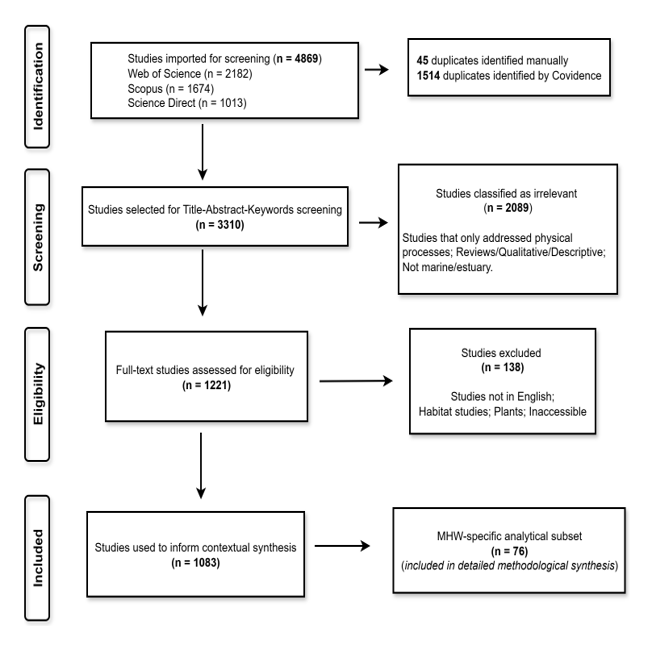
\includegraphics[width=0.9\textwidth]{lit_prisma}
\caption{PRISMA flow diagram for the literature search, screening and inclusion. Left column, records retained at each stage; right column, records removed and the reason.}
\label{fig:prisma}
\end{figure}

\subsection{Temporal dynamics of the literature}
MHW specific impact research grew steadily from 2016, peaked in 2021 with 18 studies, and has remained at 11 to 13 studies a year since (Fig.~\ref{fig:temporal}a). Citations peaked in 2021 (601) and have declined for more recent years, as expected from citation lag. The growth coincided with wider availability of satellite derived sea surface temperature and with standardised event detection software, which lowered the technical barrier to linking exposure to biological responses. Across response families, Population/Demography and Physiology/Bioenergetics drove the growth, expanding from minimal activity in 2016 to 2017 to peaks in 2021 before declining; Distribution/Range/Phenology followed a more moderate trajectory peaking around 2021 to 2022; Community/Ecosystem studies remained low and Fisheries/Economics endpoints were rarely addressed (Fig.~\ref{fig:temporal}b). The 2021 peak followed the 2014 to 2016 Northeast Pacific event, the 2015 to 2016 Tasman Sea event and the 2016 Great Barrier Reef bleaching. Whether the subsequent decline reflects an event driven research cycle or consolidation around established methods cannot be resolved from counts alone.

\begin{figure}[H]\centering
\panel{a}{0.52\textwidth}{lit_publications_citations}\hfill\panel{b}{0.46\textwidth}{lit_family_by_year}
\caption{Temporal dynamics of the MHW impact literature. (a) Annual number of publications (bars) and citations received (line), 2016 to 2025. (b) Number of studies by publication year and response family.}
\label{fig:temporal}
\end{figure}

\subsection{Collaboration structure}
Collaboration is organised around a small number of hubs (Fig.~\ref{fig:network}a). NOAA and the University of Western Australia are the most central institutions, each embedded in a dense regional cluster: the University of Tasmania, the Australian Institute of Marine Science, CSIRO and Curtin University form a coherent Australian hub, while NOAA anchors an extensive North American network of universities and federal agencies. CNRS (France), Fisheries and Oceans Canada and IMEDEA (Spain) act as secondary connectors between otherwise distinct clusters. At national scale the United States is the principal connector, with Australia, Canada, Spain and France as secondary hubs and China, Switzerland and Portugal showing substantial international linkages (Fig.~\ref{fig:network}b). The network is sparse beyond the hubs, which is consistent with the slow diffusion of specialised methods into regions without sustained institutional capacity.

\begin{figure}[H]\centering
\panel{a}{0.92\textwidth}{lit_network_institutions}\\[6pt]
\panel{b}{0.5\textwidth}{lit_network_countries}
\caption{Collaboration landscape of MHW impact studies. (a) Institutional co authorship network drawn in VOSviewer; node size is publication output, edge thickness is collaboration strength and colour identifies the cluster. (b) International co authorship as a chord diagram; ribbon width is the number of shared studies. Institutional acronyms are defined in Table~\ref{tab:acronyms}.}
\label{fig:network}
\end{figure}

\section{Literature search and classification}

\subsection{Search strings}
Table~\ref{tab:search} reproduces the search string run in each of the three primary databases. In Web of Science and Scopus six term groups were combined with AND: marine heatwave terminology (including the broader terms ocean warming and climate change), a marine scope term, impact descriptors, biological endpoints, the taxonomic term fish*, and methodological terms; terms within a group were combined with OR and truncated. Publication years were restricted to 2010 to 2025 through the PY field in Web of Science and PUBYEAR limits in Scopus. ScienceDirect, whose query syntax does not support truncation or long nested Boolean strings, was searched with a reduced string of four groups. Google Scholar and NOAA repositories were searched with the core terms as supplementary sources and were not counted in the record totals. Title and abstract screening was conducted independently by three reviewers and full text assessment by two; conflicts at either stage were resolved by consensus through discussion with the wider author group and re evaluation against the inclusion criteria. Record counts are those at retrieval; 1,559 duplicates were removed before screening (Fig.~\ref{fig:prisma}).

% GENERATED by scripts/make_literature_tables.R from data/literature/search_strategy.csv -- do not edit
\begin{table}[H]\centering
\caption{Search strings applied to each database, reproduced verbatim, with the number of records retrieved. The asterisk denotes truncation; TS, topic field (Web of Science); PY, publication year.}
\label{tab:search}\footnotesize\setlength{\tabcolsep}{4pt}
\begin{tabular}{>{\raggedright\arraybackslash}p{2.1cm}>{\raggedright\arraybackslash}p{11.6cm}r}\toprule
Database & Search string & Records \\\midrule
Web of Science & TS=(\textquotedbl{}marine heatwave*\textquotedbl{} OR \textquotedbl{}ocean heatwave*\textquotedbl{} OR \textquotedbl{}marine heat event*\textquotedbl{} OR \textquotedbl{}extreme ocean temperature*\textquotedbl{} OR \textquotedbl{}climate change\textquotedbl{} OR \textquotedbl{}ocean warming\textquotedbl{}) AND TS=(marine) AND TS=(impact* OR effect* OR response* OR \textquotedbl{}ecological consequence*\textquotedbl{} OR assessment OR sensitivity OR vulnerability) AND TS=(mortality OR growth OR abundance OR biomass OR physiology OR behavio* OR behavior* OR recruitment OR distribution OR reproduction OR survival) AND TS=(fish*) AND TS=(regression OR model* OR \textquotedbl{}data analy*\textquotedbl{} OR statistic* OR \textquotedbl{}field study\textquotedbl{} OR survey) AND PY=(2010-2025) & 2,182 \\
Scopus & (TITLE-ABS-KEY ( \textquotedbl{}marine heatwave*\textquotedbl{} OR \textquotedbl{}ocean heatwave*\textquotedbl{} OR \textquotedbl{}marine heat event*\textquotedbl{} OR \textquotedbl{}extreme ocean temperature*\textquotedbl{} OR \textquotedbl{}climate change\textquotedbl{} OR \textquotedbl{}ocean warming\textquotedbl{} ) ) AND PUBYEAR \textgreater{} 2009 AND PUBYEAR \textless{} 2026 AND ( TITLE-ABS-KEY ( marine ) ) AND ( TITLE-ABS-KEY ( impact* OR effect* OR response* OR \textquotedbl{}ecological consequence*\textquotedbl{} OR assessment OR sensitivity OR vulnerability ) ) AND ( TITLE-ABS-KEY ( mortality OR growth OR abundance OR biomass OR physiology OR behavio* OR behavior* OR recruitment OR distribution OR reproduction OR survival ) ) AND ( TITLE-ABS-KEY ( fish* ) ) AND ( TITLE-ABS-KEY ( regression OR model* OR \textquotedbl{}data analy*\textquotedbl{} OR statistic* OR \textquotedbl{}field study\textquotedbl{} OR survey ) ) & 1,674 \\
ScienceDirect & (\textquotedbl{}marine heatwave\textquotedbl{} OR \textquotedbl{}ocean warming\textquotedbl{} OR \textquotedbl{}climate change\textquotedbl{}) AND marine AND (impact OR response OR effect) AND (fisheries OR fish) & 1,013 \\
\midrule
Total before de duplication & & 4,869 \\
\bottomrule\end{tabular}\end{table}


\subsection{Response term mapping}
Free text descriptors in each study's response field were mapped to a controlled vocabulary of sub metrics and then to five response families (Population/Demography, Physiology/Bioenergetics, Distribution/Range/Phenology, Community/Ecosystem, Fisheries/Economics) with the curated regular expressions in Table~\ref{tab:regex}. Response text was pre processed (lower cased, Unicode normalised, punctuation standardised) before matching. A study measuring several responses could match several sub metrics; disambiguation rules resolved the recurring ambiguities, in particular fishery dependent abundance (CPUE, landings, effort) against economic outcomes, and spatial behaviour (home range, space use) against non spatial behaviour (activity, foraging). The rule set is deposited with the repository as \texttt{data/literature/response\_term\_mapping.csv} and the table is typeset from that file, so every assignment can be re run.

% GENERATED by scripts/make_literature_tables.R from data/literature/response_term_mapping.csv -- do not edit
\begin{footnotesize}
\setlength{\tabcolsep}{4pt}
\begin{longtable}{>{\raggedright\arraybackslash}p{5.4cm}>{\raggedright\arraybackslash}p{5.1cm}>{\raggedright\arraybackslash}p{2.2cm}>{\raggedright\arraybackslash}p{2.0cm}}
\caption{Regex patterns for mapping response terms to standardised submetrics and response families. Raw terms are those extracted from the studies' response fields; patterns were applied case insensitively.}\label{tab:regex}\\
\toprule
Raw terms & Matched regex & Submetric & Family \\
\midrule
\endfirsthead
\multicolumn{4}{l}{\small Table~\thetable{} (continued)}\\
\toprule
Raw terms & Matched regex & Submetric & Family \\
\midrule
\endhead
\midrule \multicolumn{4}{r}{\small continued on next page}\\
\endfoot
\bottomrule
\endlastfoot
Biomass; biomass changes; biomass decline; ecosystem biomass decline; spawning biomass; Trophic-\allowbreak{}Level-\allowbreak{}specific sensitivity; trophic response; Fish biomass & \texttt{biomass\allowbreak{}( changes)?|\allowbreak{}trophic\allowbreak{}(-|\allowbreak{} )level |\allowbreak{} trophic response |\allowbreak{} productivity |\allowbreak{} ecosystem biomass decline |\allowbreak{} recovery times |\allowbreak{} survey biomass distribution} & Biomass/\allowbreak{}Productivity & Community/\allowbreak{}Ecosystem \\
Community composition; Diversity; diversity changes; diversity indices; fish assemblage; functional group response; functional group shifts; functional richness; richness; species assemblage; species richness & \texttt{Diversity |\allowbreak{} richness |\allowbreak{} evenness |\allowbreak{} functional \allowbreak{}(richness |\allowbreak{} group |\allowbreak{}response) |\allowbreak{}community composition |\allowbreak{} assemblage} & Diversity/\allowbreak{}Composition &  \\
Asynchrony; Community shifts; community shifts; community stability; Deborealization signals; food web restructuring; resilience; resilience under protection; Tropicalization patterns; Tropicalization signals & \texttt{stability|\allowbreak{}asynchrony|\allowbreak{}resilience|\allowbreak{}tropicalization|\allowbreak{}deborealization|\allowbreak{}community shifts |\allowbreak{} food web restructuring} & Stability/\allowbreak{}Function &  \\
\addlinespace
distribution; distribution shifts; Distribution; area occupied; Centre of mass depth; Centroids of distribution in depth; depth distribution; Depth of occurrence; distribution patterns; Distribution shift; distributions; habitat distribution shifts; latitude; longitude; redistribution Shifts in center of gravity; size distribution; Species-\allowbreak{}specific spatial distribution; survey biomass distribution under scenarios; Vertical distribution & \texttt{Distribution \allowbreak{}( shifts |\allowbreak{} patterns)? |\allowbreak{} redistribution |\allowbreak{}centroid |\allowbreak{}center of gravity |\allowbreak{}area occupied |\allowbreak{} latitude |\allowbreak{} longitude |\allowbreak{} vertical distribution |\allowbreak{} depth distribution |\allowbreak{} centre of mass depth |\allowbreak{} mesopelagic patch size |\allowbreak{} depth of occurrence} & Distribution (2D/\allowbreak{}Depth) & Distribution/\allowbreak{}Range/\allowbreak{}Phenology \\
habitat suitability; habitat loss impacts; habitat quality; Habitat suitability; habitat use; port availability; projected habitat suitability & \texttt{habitat \allowbreak{}(use |\allowbreak{} quality |\allowbreak{} loss) |\allowbreak{} habitat suitability |\allowbreak{} projected habitat suitability |\allowbreak{} environmental habitat associations |\allowbreak{} port availability} & Habitat/\allowbreak{}Habitat Suitability &  \\
Migration routes & \texttt{migration routes |\allowbreak{} home range |\allowbreak{} space use |\allowbreak{} diel overlap} & Movement/\allowbreak{}Space use &  \\
Phenology; phenology; phenology shifts; spawning shifts & \texttt{Phenology |\allowbreak{} hatch timing |\allowbreak{} spawning shifts |\allowbreak{} timing} & Phenology &  \\
biogeographic shifts; Poleward range shifts; range expansion; range shift; Range shift persistence & \texttt{range shift |\allowbreak{}range expansion |\allowbreak{}biogeographic shifts |\allowbreak{}poleward range} & Range change &  \\
\addlinespace
food security risks; revenue shocks & \texttt{Revenue |\allowbreak{} profit |\allowbreak{} price\allowbreak{}(s)? |\allowbreak{} income |\allowbreak{} food security |\allowbreak{} employment |\allowbreak{} cost\allowbreak{}(s)? |\allowbreak{} market |\allowbreak{} economic |\allowbreak{} livelihood} & Revenue/\allowbreak{}Markets/\allowbreak{}Food security & Fisheries/\allowbreak{}Economics \\
\addlinespace
Activity level; behaviour; diel behavior; grazing; swimming performance & \texttt{activity level |\allowbreak{} behaviour |\allowbreak{}foraging |\allowbreak{} grazing |\allowbreak{} swimming performance |\allowbreak{} avoidance |\allowbreak{} boldness |\allowbreak{} diel} & Behaviour/\allowbreak{}Performance & Physiology/\allowbreak{}Bioenergetics \\
energy budget; feed efficiency; Flesh colour; Nutritional quality; tissue quality & \texttt{energy budget |\allowbreak{} feed efficiency |\allowbreak{} flesh colour |\allowbreak{} tissue quality |\allowbreak{} nutritional quality} & Bioenergetics/\allowbreak{}Quality &  \\
age-\allowbreak{}0 body condition; body condition; Residual Condition Index of selected fish & \texttt{body condition |\allowbreak{} condition index |\allowbreak{} residual condition} & Condition &  \\
growth; Growth; growth patterns; growth performance; Growth rates; growth trajectories; relative growth rate & \texttt{Growth \allowbreak{}(rate |\allowbreak{} trajectories |\allowbreak{} patterns)? |\allowbreak{} relative growth rate} & Growth &  \\
antioxidant activity; immune health; immune responses; lysozyme & \texttt{Immune |\allowbreak{} igm |\allowbreak{} lysozyme |\allowbreak{} antioxidant} & Immunity &  \\
Aerobic metabolism; excretion; metabolic rate; metabolism; oxygen consumption; respiration; routine metabolic rate & \texttt{metaboli\allowbreak{}(c|\allowbreak{}sm) |\allowbreak{} respiration |\allowbreak{} excretion |\allowbreak{} oxygen consumption |\allowbreak{} routine metabolic} & Metabolism &  \\
DNA methylation patterns (DMRs); environmental habitat associations; gene expression; gene expression in tissues; home range shifts; mesopelagic patch size; metabolomic pathways; metastable epialleles (MEs); mitigation from mesophotic refuges; recovery times; transcriptome & \texttt{gene expression |\allowbreak{} transcriptome |\allowbreak{} dna methylation |\allowbreak{} epigenetic |\allowbreak{} dmr |\allowbreak{} me\allowbreak{}(s)?} & Molecular/\allowbreak{}Epigenetic &  \\
acclimation capacity; CTmax; Physiological stress; thermal tolerance thresholds & \texttt{Ctmax |\allowbreak{} thermal tolerance |\allowbreak{} physiological stress |\allowbreak{} acclimation capacity} & Thermal/\allowbreak{}Stress Tolerance &  \\
\addlinespace
CPUE; Catch; Bycatch rates; catch; Catch and Effort; CPUE catchability; effort; fleet-\allowbreak{}specific catchability shifts; Length-\allowbreak{}at-\allowbreak{}catch distribution; maximum catch potential; Probability of occurrence by fleet; Spatial catch & \texttt{Cpue |\allowbreak{} catchability |\allowbreak{}catch\allowbreak{}(,|\allowbreak{};|\allowbreak{}\$|\allowbreak{} ) |\allowbreak{} effort |\allowbreak{} landings |\allowbreak{} bycatch |\allowbreak{} fleet} & Abundance/\allowbreak{}CPUE (fishery-\allowbreak{}dependent) & Population/\allowbreak{}Demography \\
Abundance; abundance; abundance shifts; Abundance (CPUE); densities; density; density changes; Fish abundance; fish densities; juvenile abundance; larval abundance; Species abundance; standardized abundance; temperature \& abundance relationships; Urchin density & \texttt{Abundance |\allowbreak{} juvenile abundance |\allowbreak{} standardized abundance |\allowbreak{} densit\allowbreak{}(y|\allowbreak{}ies)} & Abundance/\allowbreak{}Density &  \\
survival; Survival; mortality; Mortality thresholds; Calf mortality; Embryo survival; extirpation risk; potential selective mortality; survival under harvesting + MHW stress & \texttt{Mortality |\allowbreak{}extirpation risk |\allowbreak{} survival\allowbreak{}(?!.*post)} & Mortality/\allowbreak{}Survival &  \\
recruitment; recruitment failure; recruitment failure mechanisms; recruitment indeces; recruitment index; recruitment patterns; recruitment success; Recruitment variation & \texttt{Recruitment \allowbreak{}(index |\allowbreak{} failure |\allowbreak{} patterns |\allowbreak{} success |\allowbreak{} variation)?} & Recruitment &  \\
Calf production; Egg buoyancy; hatch timing; Hatch timing; pup numbers; reproductive output; spawning stock biomass & \texttt{reproductive output |\allowbreak{} egg |\allowbreak{} larval |\allowbreak{} hatch |\allowbreak{} calf |\allowbreak{} pup |\allowbreak{} spawning stock biomass |\allowbreak{} embryo} & Reproduction/\allowbreak{}Early life &  \\
length frequency; population structure; size structure; size structure (length classes) & \texttt{size structure |\allowbreak{} length \allowbreak{}(frequency |\allowbreak{} classes) |\allowbreak{} population structure |\allowbreak{} age structure} & Size/\allowbreak{}Age Structure &  \\
\end{longtable}
\end{footnotesize}


\subsection{Institutional acronyms}
\begin{table}[H]\centering
\caption{Institutional acronyms used in Fig.~\ref{fig:network}.}
\label{tab:acronyms}\small
\begin{tabular}{ll}\toprule
Acronym & Institution \\\midrule
AIMS & Australian Institute of Marine Science \\
CNRS & Centre National de la Recherche Scientifique, France \\
CSIRO & Commonwealth Scientific and Industrial Research Organisation, Australia \\
DFO & Fisheries and Oceans Canada \\
IMEDEA & Mediterranean Institute for Advanced Studies, Spain \\
NOAA & National Oceanic and Atmospheric Administration, United States \\
UCSC & University of California, Santa Cruz \\
UTAS & University of Tasmania \\
UWA & University of Western Australia \\
\bottomrule\end{tabular}\end{table}

\section{Detection verification and sensitivity}

\subsection{Reference values}
Table~\ref{tab:detref} gives the characteristics of the most intense event (by peak anomaly) in each of the three real OISST series under the Hobday defaults, as computed by heatwaveR \heatwaveRVersion{} on R \rVersion{}. These are the reference values against which the repository's test suite checks; they are regenerated on the analyst's machine by \texttt{scripts/verify\_detection.R}.

\detectionReferenceTable

\subsection{Sensitivity of the 2011 Western Australian event}
Table~\ref{tab:detsens} shows how the 2011 event's characteristics change across three climatology windows and two percentile thresholds. The event is robust to the 95th percentile and to extending the window to 2022, but under a 1982 to 2011 window at the 90th percentile the detection algorithm joins the 2011 anomaly to a different event structure and the largest 2011 event by peak anomaly becomes a short November event. This is the sensitivity that item 2 of the reporting standards asks authors to disclose.

\detectionSensitivityTable

\begin{figure}[H]\centering
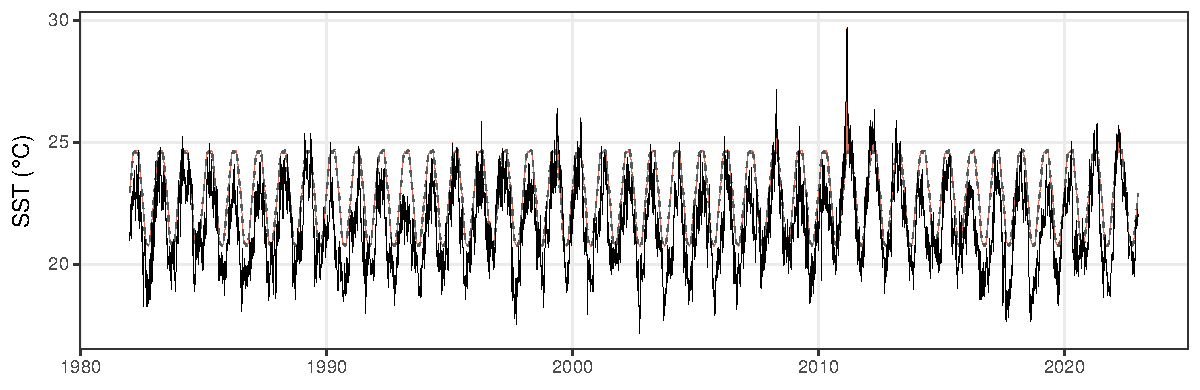
\includegraphics[width=\textwidth]{fig_detection_wa_series}
\caption{Daily OISST for the Western Australian series, 1982 to 2022 (black), the 90th percentile threshold (dashed grey) and exceedance above threshold (shaded) for every detected event. The 2011 event is the tallest exceedance; the 1999 event, longer but lower, is the largest by cumulative intensity.}
\label{fig:detection}
\end{figure}

\section{Data generating process calibration}
Table~\ref{tab:dgp} reports the realised response distribution for every combination of true effect and true lag on one 9 site and one 25 site panel per region (range 50 km, replicate 1). All cells are usable: no cell has more than 90\% zeros, fewer than five distinct values, or an implausible mean.

\dgpCalibrationTable

\section{Full simulation results}
This section gives every aggregation of the simulation output on which the main text draws. All tables are generated from \texttt{results/tables/} by \texttt{scripts/make\_supp\_tables.R}; the raw file \texttt{R\_raw\_results.csv} (one row per model fit) is deposited with the repository. Model classes are described in Table 4 of the main text; the estimand reported as $\hat\beta_1$ differs between classes as stated there.

\subsection{Model level summary}
Table~\ref{tab:modsum} averages over all \nScenarios{} scenarios. The ordering by RMSE places the two GLMs ahead of the DLNM because their estimates, although biased, vary little across replicates; the ordering by mean bias places the DLNM first. Coverage and log score are averaged only over scenarios where the quantity is defined (no interval for the random forest; no proper predictive density for the quasi Poisson DLNM). The sdmTMB row summarises the \sdmtmbPanelsN{} panels on which that model was run.
\modelSummaryTable

\subsection{Bias by true lag}
Table~\ref{tab:biaslag} is the breakdown behind Fig.~5 of the main text. The naive GLM's bias changes sign between lag 0 and lag 1 and stays at that level at lag 2; the lag-1 GLM shows the mirror image, small at lag 1 and large at lags 0 and 2; the DLNM's bias stays within a narrow band at all three lags but with a larger standard deviation across replicates.
\biasByLagTable

\subsection{Relative bias by true effect and lag}
Table~\ref{tab:relbias} expresses the same biases as a percentage of the true coefficient (Fig.~6 of the main text). Because the absolute bias under lag misspecification is approximately constant, the percentage is largest for the smallest true effect ($\beta_1 = -0.04$), where the naive GLM's estimate can exceed the true magnitude in the wrong direction at lag 0 and vanish entirely at lags 1 and 2.
\relativeBiasTable

\subsection{Bias by region}
Table~\ref{tab:biasregion} is the breakdown behind Fig.~9 of the main text. Regional exposure distributions differ substantially (mean annual cumulative intensity of roughly 20, 50 and 40\,$^{\circ}$C days for the Western Australian, Northwest Atlantic and Mediterranean series; Table~\ref{tab:dgp}), yet the bias of each model class is nearly constant across regions, which is what is expected when the bias arises from the model's temporal assumption rather than from the exposure values.
\biasByRegionTable

\subsection{Bias by grid size and spatial range}
Table~\ref{tab:biasgeom} splits the results by the two spatial design factors. Neither factor changes the bias of any class detectably. The number of sites changes precision (RMSE falls from 9 to 25 sites for the classes whose estimates are unbiased at the correct lag), and the correlation range changes nothing, because the site effects absorb the correlated component of the exposure noise.
\biasByGeometryTable

\subsection{Convergence and runtime}
Table~\ref{tab:runreport} is the run report printed by \texttt{scripts/aggregate.R}. The percentage returning an estimate and the percentage passing the package's own convergence check are reported separately: a fit that triggered a warning (for the GLMs, typically the theta iteration limit in \texttt{glm.nb}; for sdmTMB, a non positive definite Hessian reported by \texttt{sanity()}) was retained with its estimate and counted as not converged, rather than being dropped. Median runtime per fit is on one core; package versions are given in Section 3.3 of the main text and the full \texttt{sessionInfo()} output is deposited with the repository as \texttt{results/tables/sessionInfo.txt}.
\runReportTable

\subsection{Additional figures}
Figures~\ref{fig:srmse} and \ref{fig:smorans} complement the main text figures. The RMSE figure shows the precision cost of the DLNM's robustness: its boxes are wider than the correctly lagged GLM's at every lag. The Moran's $I$ figure shows that residual spatial autocorrelation is small and slightly negative for every regression class on both independent and correlated panels, which confirms that the correlated exposure noise is absorbed by the site effects and leaves no spatial structure for a random field model to explain.

\begin{figure}[H]\centering
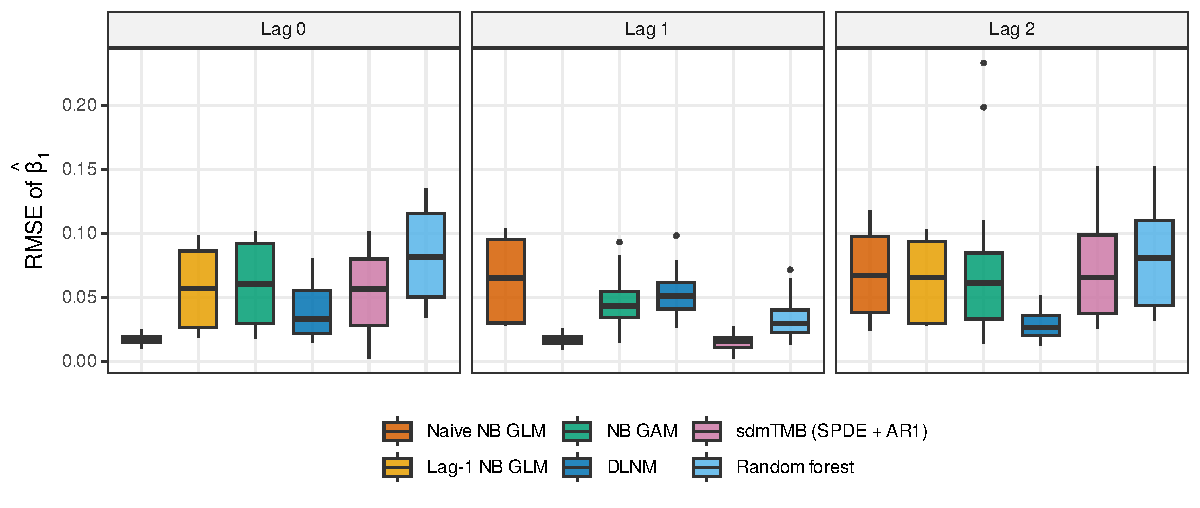
\includegraphics[width=\textwidth]{fig_rmse}
\caption{Root mean squared error of the estimated exposure coefficient by model class and true lag; each box summarises one third of the \nScenarios{} scenarios. Colours identify model classes consistently with the main text.}
\label{fig:srmse}
\end{figure}

\begin{figure}[H]\centering
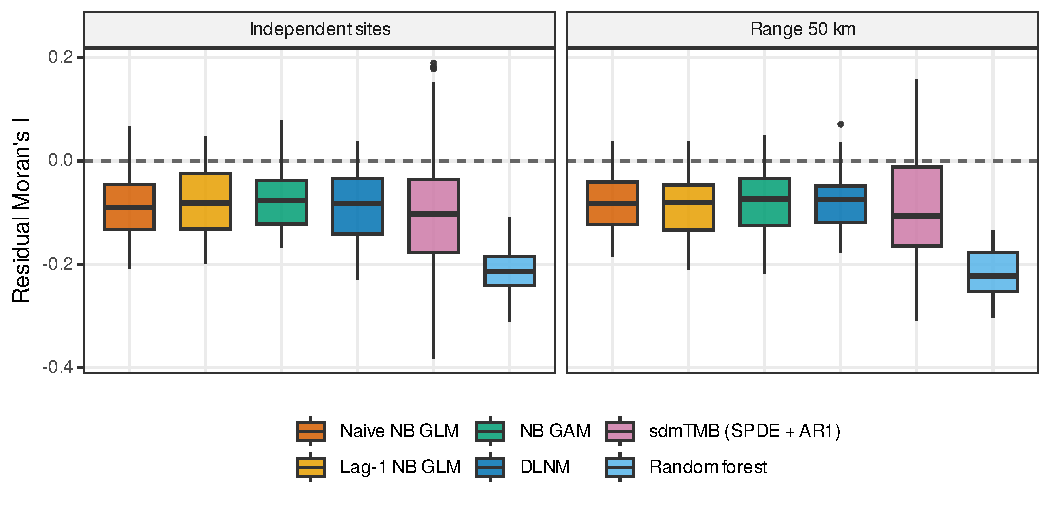
\includegraphics[width=0.8\textwidth]{fig_morans}
\caption{Residual Moran's $I$ of site mean residuals by model class, for spatially independent panels and panels with a 50 km correlation range.}
\label{fig:smorans}
\end{figure}

\section{Repository structure and reproduction}
\begin{lstlisting}[language={}]
mhw-R-audit/
  R/00_config.R      design constants, seeds, paths
  R/01_detection.R   heatwaveR wrappers
  R/02_exposure.R    annual metrics, lag panels
  R/03_panel.R       OISST loader, Matern spatial panel
  R/04_dgp.R         response simulator, degeneracy checks
  R/05_models.R      six fitters, unified return interface
  R/06_runner.R      resumable checkpointed runner
  R/07_aggregate.R   summaries, run report
  scripts/verify_detection.R    RUN FIRST: reference values
  scripts/diagnose_dgp.R        RUN SECOND: calibration check
  scripts/run_chunk.R           one array task
  scripts/aggregate.R           summaries
  scripts/make_figures.R        figures
  scripts/make_results_macros.R manuscript macros
  scripts/make_main_tables.R    main text tables
  scripts/make_supp_tables.R    supplement tables
  scripts/make_literature_tables.R  Tables S1 and S2 from data/literature
  scripts/prepare_literature_figures.R  stage the synthesis figure panels
  data/literature/search_strategy.csv          search strings (Table S1)
  data/literature/response_term_mapping.csv   response term rules (Table S2)
  hpc/slurm_array.sh, hpc/pbs_array.sh, hpc/run_local_parallel.sh
  tests/testthat/test-detection.R
  manuscript/main.tex, supplement.tex, refs.bib
\end{lstlisting}

Reproduction on a workstation:
\begin{lstlisting}[language=bash]
export MHW_ROOT=$PWD
Rscript install/install_packages.R --all
Rscript scripts/verify_detection.R
Rscript scripts/diagnose_dgp.R
Rscript -e 'library(testthat); test_dir("tests/testthat")'
bash hpc/run_local_parallel.sh 8
Rscript scripts/make_results_macros.R
cd manuscript && latexmk -pdf main.tex supplement.tex
\end{lstlisting}

\section{Model fitter interface}
Every fitter in \texttt{R/05\_models.R} returns the same fields, so that a new model can be added without changing the runner:
\begin{lstlisting}
fit_<model>(d)   # d: y, site, year, X, Y, i_cum, i_cum_lag0..3, mhw_days
# returns list(model_id, beta1_hat, beta1_lo, beta1_hi,
#              log_score, morans_I, converged, runtime_sec, note)
\end{lstlisting}
The sdmTMB fitter illustrates the convention for convergence reporting: warnings are muffled rather than treated as failure, and the package's own \texttt{sanity()} verdict is recorded so that flagged fits enter the run report rather than vanishing as missing rows.
\begin{lstlisting}
m <- withCallingHandlers(
  sdmTMB::sdmTMB(y ~ i_cum_lag1, data = tr, mesh = mesh, time = "year",
                 family = sdmTMB::nbinom2(link = "log"),
                 spatial = "on", spatiotemporal = "ar1", silent = TRUE),
  warning = function(w) invokeRestart("muffleWarning"))
converged <- isTRUE(sdmTMB::sanity(m, silent = TRUE)$all_ok)
\end{lstlisting}

\bibliography{refs}
\end{document}
